\documentclass[a4paper,14pt]{extreport}
\usepackage[left=1.5cm,right=1.5cm,
    top=1.5cm,bottom=2cm,bindingoffset=0cm]{geometry}
\usepackage{scrextend}
\usepackage[T1,T2A]{fontenc}
\usepackage[utf8]{inputenc}
\usepackage[english,russian,ukrainian]{babel}
\usepackage{tabularx}
\usepackage{amssymb}
\usepackage{color}
\usepackage{amsmath}
\usepackage{mathrsfs}
\usepackage{listings}
\usepackage{graphicx}
\graphicspath{ {./images/} }
\usepackage{lipsum}
\usepackage{xcolor}
\usepackage{hyperref}

\usepackage{tcolorbox}
\usepackage{tikz}
\usepackage[framemethod=TikZ]{mdframed}
\usepackage{wrapfig,boxedminipage,lipsum}
\mdfdefinestyle{MyFrame}{%
linecolor=blue,outerlinewidth=2pt,roundcorner=20pt,innertopmargin=\baselineskip,innerbottommargin=\baselineskip,innerrightmargin=20pt,innerleftmargin=20pt,backgroundcolor=gray!50!white}
 \usepackage{csvsimple}
 \usepackage{supertabular}
\usepackage{pdflscape}
\usepackage{fancyvrb}
%\usepackage{comment}
\definecolor{ggreen}{rgb}{0.,1,0}
\definecolor{rred}{rgb}{1,0.1,0.1}
\usepackage{array,tabularx}
\usepackage{colortbl}

\usepackage{varwidth}
\tcbuselibrary{skins}
\usepackage{fancybox}




\usepackage{float}
\usepackage{wrapfig}
\usepackage{framed}





\begin{document}
\renewcommand{\bibname}{Список використаної літератури}
\pagecolor{white}
\begin{titlepage}
  \begin{center}
    \large
    Національний технічний університет України \\ "Київський політехнічний інститут імені Ігоря Сікорського"


    Факультет Електроніки

    Кафедра мікроелектроніки
    \vfill

    \textsc{ЗВІТ}\\

    {\Large Про виконання домашньої контрольної роботи\\
      з дисципліни: «Твердотільна електроніки-1»\\[1cm]



    }
  \bigskip
\end{center}
\vfill

\newlength{\ML}
\settowidth{\ML}{«\underline{\hspace{0.4cm}}» \underline{\hspace{2cm}}}
\hfill
\begin{minipage}{1\textwidth}
Виконавець:\\
Студент 3-го курсу \hspace{4cm} $\underset{\text{(підпис)}}{\underline{\hspace{0.2\textwidth}}}$  \hspace{1cm}А.\,С.~Мнацаканов\\
\vspace{1cm}

Перевірив: \hspace{6.1cm} $\underset{\text{(підпис)}}{\underline{\hspace{0.2\textwidth}}}$  \hspace{1cm}О.\,В.~Борисов\\

\end{minipage}

\vfill

\begin{center}
2020
\end{center}
\end{titlepage}


%--------------------------------------------------------------------------------------1-----------------------------------------------------------------------------------------
\tableofcontents

%--------------------------------------------------------------------------------------2-----------------------------------------------------------------------------------------
\newpage
\begin{center}\bf{\Large{Основні позначення}}\end{center}\par

$U_{\text{зв}}$ --- максимально допустима постійна зворотна напруга на діоді.\\

$U_{\text{зв імп}}$ --- максимально допустима постійна імпульсна зворотна напруга на діоді.\\

$U_{\text{пр}}$ --- максимальне падіння напруги на діоді при заданому прямому струмі ($I_{\text{пр}}$) через нього.\\

$U_{\text{пр імп}}$ --- максимально допустима постійна імпульсна прама напруга на діоді.\\

$P_{\text{}}$ --- максимально допустима постійна розсіювальна потужність.\\

$P_{\text{т}}$ --- максимально допустима постійна розсіювальна потужність на пристрою з тепловідводом.\\

$T_{\text{відн. зв.}}$ --- час зворотного відновлення.\\

$C_{\text{D}}$ --- загальна ємність.\\

$U_{\text{ст}}$ --- напруга стабілізації.\\

$Q_{\text{}}$ --- добротність елемента.\\

$F_{\text{d}}$ --- робоча частота діода.\\

$F_{\text{max}}$ --- максимальна робоча частота діода.\\

$I_{\text{пр}}$ --- максимально допустимий постійний прямий струм через діоді.\\

$I_{\text{ст}}$ --- струм стабілізації.\\

$I_{\text{пр імп}}$ --- максимально допустимий постійний імпульсний прямий струм через діоді.\\

$I_{\text{зв}}$ --- максимально зворотний струм через діод при максимальній зворотній напрузі.\\

$I_{\text{зв імп}}$ --- максимально зворотний импульсний струм через діод при максимальній зворотній напрузі.\\

$K_{\text{c}}$ --- коефіцієнт перекриття по ємності варикапа при зміні напруги від U1 до U2;\\

Перший елемент - буква або цифра, що позначає вихідний матеріал:\\

1 або Г - германій або його сполуки; \\

2 або К - кремній або його сполуки; \\

3 або А - з'єднання галію.  \\

Другий елемент буква, харак теризують підклас приладу:\\
\begin{itemize}
\item  Д - діоди;
\item  Ц - випрямляючі стовпи і блоки;
\item  А - діоди СВЧ;
\item  В - варикапи;
\item  И - діоди тунельні;
\item  Н - тиристори діодні;
\item  У - тиристори тріодні;
\item  Л - випромінювачі;
\item  Г - генератори шуму;
\item  Б - діоди Ганна;
\item  К - стабілізатори струму;
\item  С - стабілітрони і стабістори. \\
\end{itemize}

Третій елемент --- число, яке вказує призначення і якісні властивості приладу, а також порядковий номер розробки.
\newpage

%--------------------------------------------------------------------------------------4-----------------------------------------------------------------------------------------
\newpage
\chapter{Діоди}
\section{Випрямні діоди}

\begin{tcolorbox}[colback=white!100,colframe=red!75!black,width=19cm,righttitle=0.5cm,subtitle style={boxrule=0.4pt, colback=yellow!50!red!25!white},title= \bf{Графічне позначення}\hfill  \bf{Натуральне зоображення}]
	\begin{center}\bf{КД202А}\end{center}
	\tcblower
	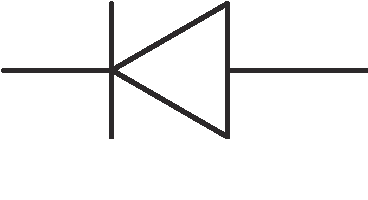
\includegraphics[scale=0.5]{1.1.pdf}\hfill 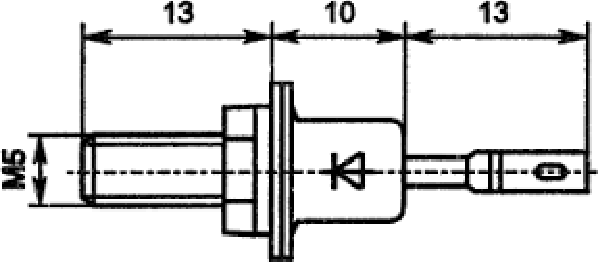
\includegraphics[scale=0.5]{1.12.pdf} \hfill\includegraphics[scale=0.3]{1.13.png}
\end{tcolorbox}

\newtcbox{\xmybox}[1][red]{on line, arc=7pt,colback=#1!10!white,colframe=#1!50!black, before upper={\rule[-3pt]{0pt}{10pt}},boxrule=1pt, boxsep=0pt,left=6pt,right=6pt,top=2pt,bottom=2pt}


\begin{wrapfigure}[0]{r}{12cm}
\vspace{-0.7 cm}
\parbox{12cm}{%
  \begin{tcolorbox}[width=12cm,right=0.5cm]
  Виробляється в металлоскляному корпусі з жорсткими виводами. Маса діода не більше 5,2 г, з комплектуючими деталями не більше 7 г.\\Діод КД202А розшифровується:
  \begin{itemize}
  \item К - матеріал, кремній; \item Д - діод випрямний (дифузійний); \item 202 - призначення і номер розробки; \item А - різновид;
  \end{itemize}
  \end{tcolorbox}}
\end{wrapfigure}

\vspace{0.5 cm}\par
\xmybox[green]{$F_{\text{max}}  =    1,2 \text{ кГц}$}\par
\vspace{0.2 cm}\par
\xmybox[green]{$I_{\text{зв}}   < 0,8\text{ мА}$}\par
\vspace{0.2 cm}\par
\xmybox[green]{$U_{\text{пр}}  =     0,9\text{ В}$}\par
\vspace{0.2 cm}\par
\xmybox[green]{$U_{\text{імп}}   =   50   \text{ В}$}\par
\vspace{0.2 cm}\par
\xmybox[green]{$U_{\text{зв}}  =   35    \text{ В}$}\par
\vspace{0.2 cm}\par
\xmybox[green]{$I_{\text{імп}}  =    9 \text{ А}$}
\vspace{0.2 cm}\par
\xmybox[green]{$I_{\text{пр}}  =    5 \text{ А}$}\par
\vspace{0.2 cm}\par
\begin{figure}[h!]\label{im1}
\begin{center}
	\begin{minipage}[h!]{0.524\linewidth}
		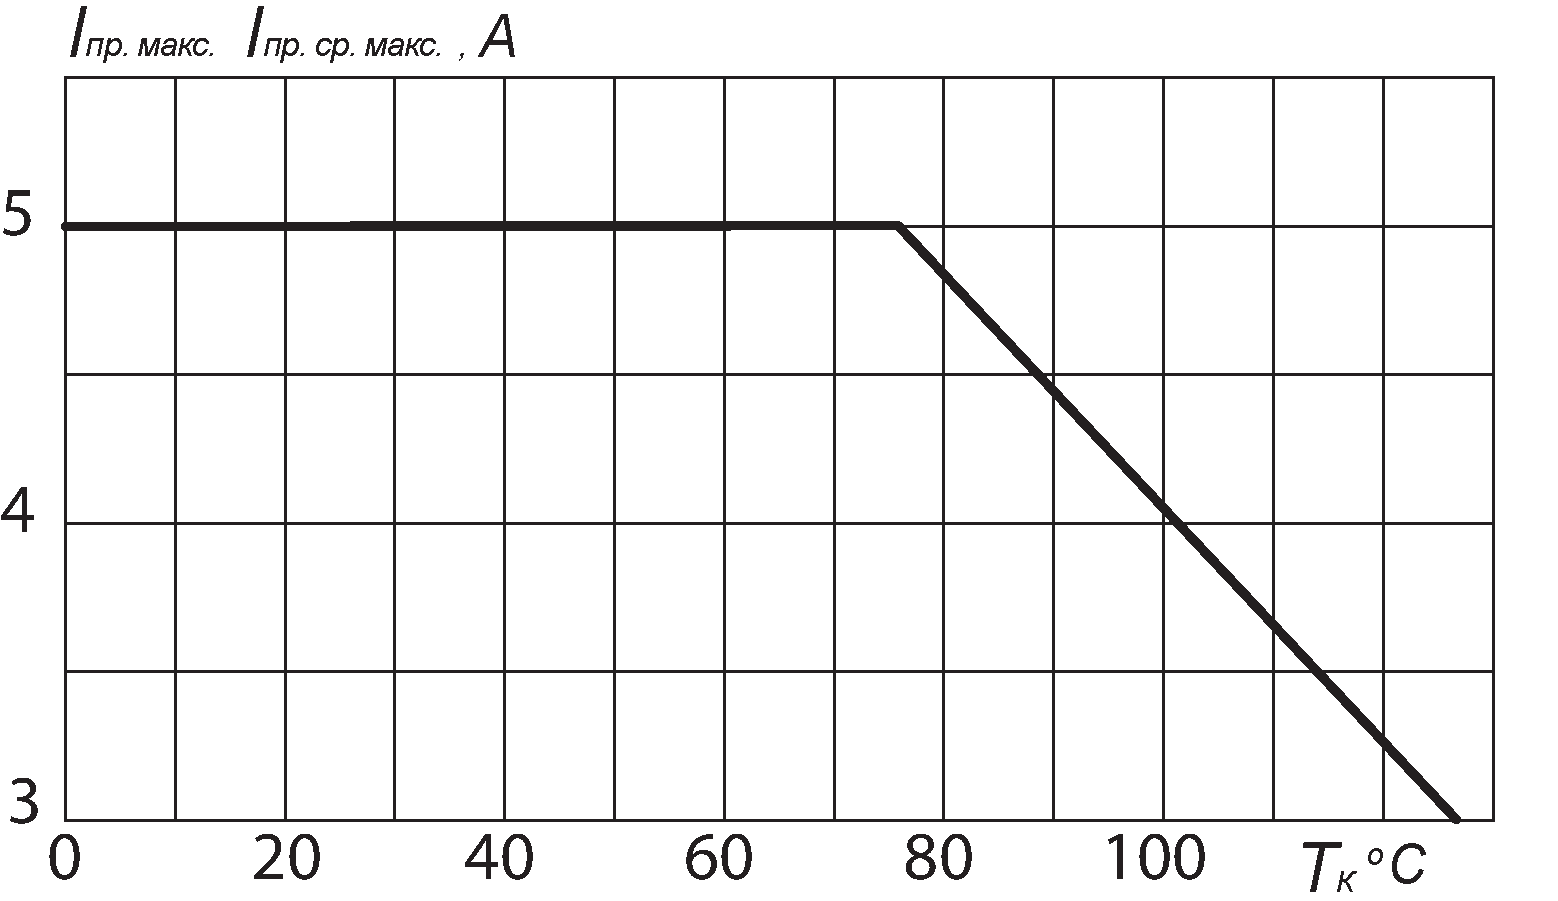
\includegraphics[width=1\linewidth]{1.17.pdf} \\
	\end{minipage}
\end{center}
\caption{Залежність допустимого прямого струму від температури корпуса.}
\end{figure}



%\tcbox[colback=green!5!white, colframe=green!50!black]{asvsdfvsd\\lsidfnb}
  %----------------------5----------------------------------------
\newpage
\begin{center}\ovalbox{Зона можливих положень залежності прямого струму від напруги за різних T}\end{center}
\begin{figure}[h!]\label{im12}
	\begin{minipage}[h]{0.524\linewidth}
		\includegraphics[width=1\linewidth]{1.15.pdf}
  \end{minipage}
\hfill
  \begin{minipage}[h]{0.524\linewidth}
		\includegraphics[width=1\linewidth]{1.16.pdf}
	\end{minipage}
\end{figure}
  \begin{figure}[h!]\label{im2}
  \begin{center}
	\begin{minipage}[h!]{0.524\linewidth}
		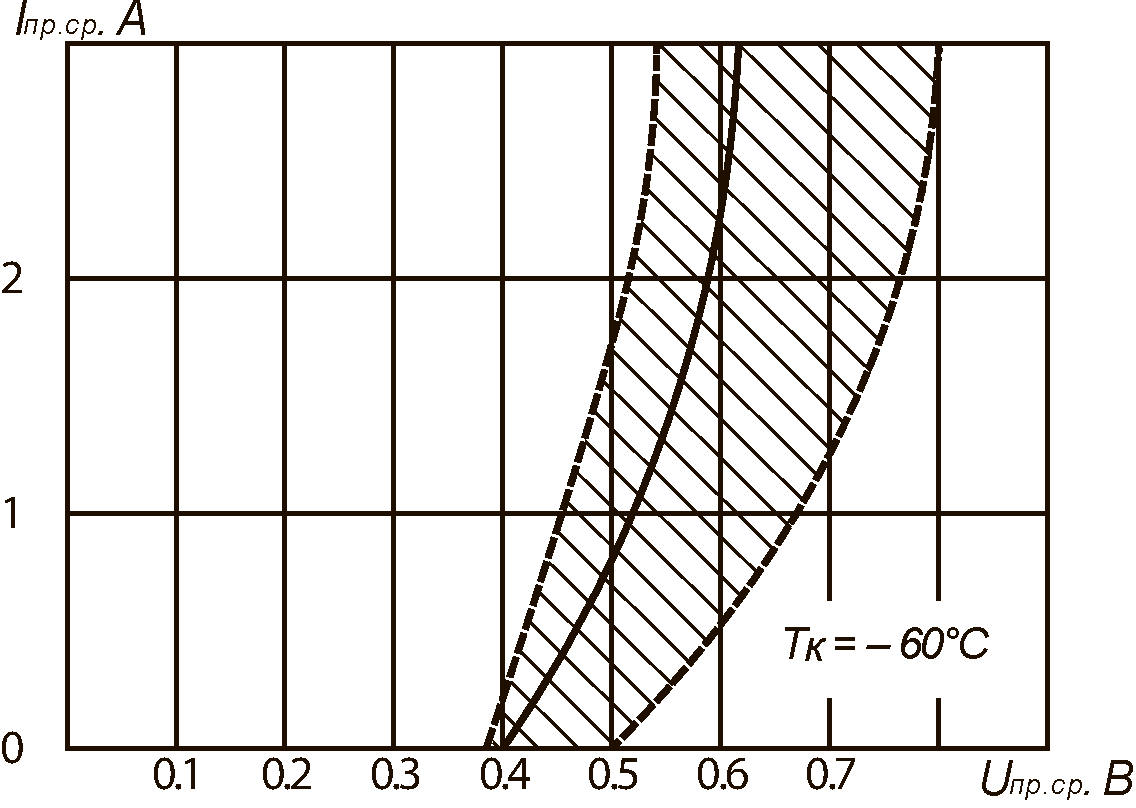
\includegraphics[width=1\linewidth]{1.14.pdf} \\
	\end{minipage}
\end{center}
\end{figure}


%-----------------------------5-----------------------------------
\newpage
\begin{tcolorbox}[colback=white!100,colframe=red!75!black,width=19cm,righttitle=0.5cm,subtitle style={boxrule=0.4pt, colback=yellow!50!red!25!white},title= \bf{Графічне позначення}\hfill  \bf{Натуральне зоображення}]
	\begin{center}\bf{Д302}\end{center}
	\tcblower
	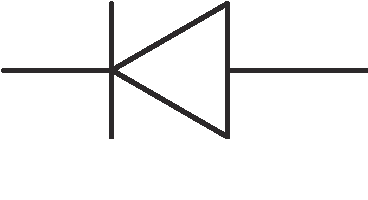
\includegraphics[scale=0.5]{1.1.pdf}\hfill 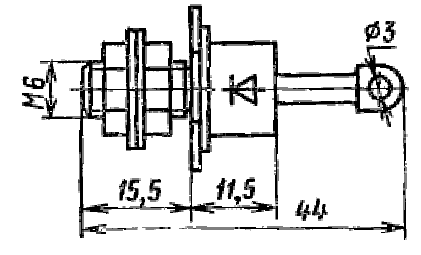
\includegraphics[scale=0.6]{1.18.pdf} \hfill\includegraphics[scale=0.3]{1.19.pdf}
\end{tcolorbox}
\begin{wrapfigure}[0]{r}{12cm}
\vspace{-0.7 cm}
\parbox{12cm}{%
  \begin{tcolorbox}[width=12cm,right=0.5cm]
  Діод германієвий, сплавний. Випускається в металлоскляному корпусі з жорсткими виводами. Маса діода не більше 16 г.
  Допускається послідовне і паралельне з'єднання діодів. При послідовному з'єднанні кожен діод повинен шунтуватися резистором опором 10...15 кОм. При паралельному з'єднанні слід підбирати діоди з близькими значеннями прямого падіння напруги.
  \end{tcolorbox}}
\end{wrapfigure}

\vspace{0.5 cm}\par
\xmybox[green]{$F_{\text{max}}  =    1 \text{ кГц}$}\par
\vspace{0.2 cm}\par
\xmybox[green]{$I_{\text{зв}}   < 0,8\text{ мкА}$}\par
\vspace{0.2 cm}\par
\xmybox[green]{$U_{\text{пр}}  =     0,3 \text{ В}$}\par
\vspace{0.2 cm}\par
\xmybox[green]{$U_{\text{зв}}  =   200    \text{ В}$}\par
\vspace{0.2 cm}\par
\xmybox[green]{$I_{\text{пр}}  =    1 \text{ А}$}\par
\vspace{0.5 cm}\par

\begin{figure}[h!]\label{im3}
	\begin{minipage}[h]{0.5\linewidth}
		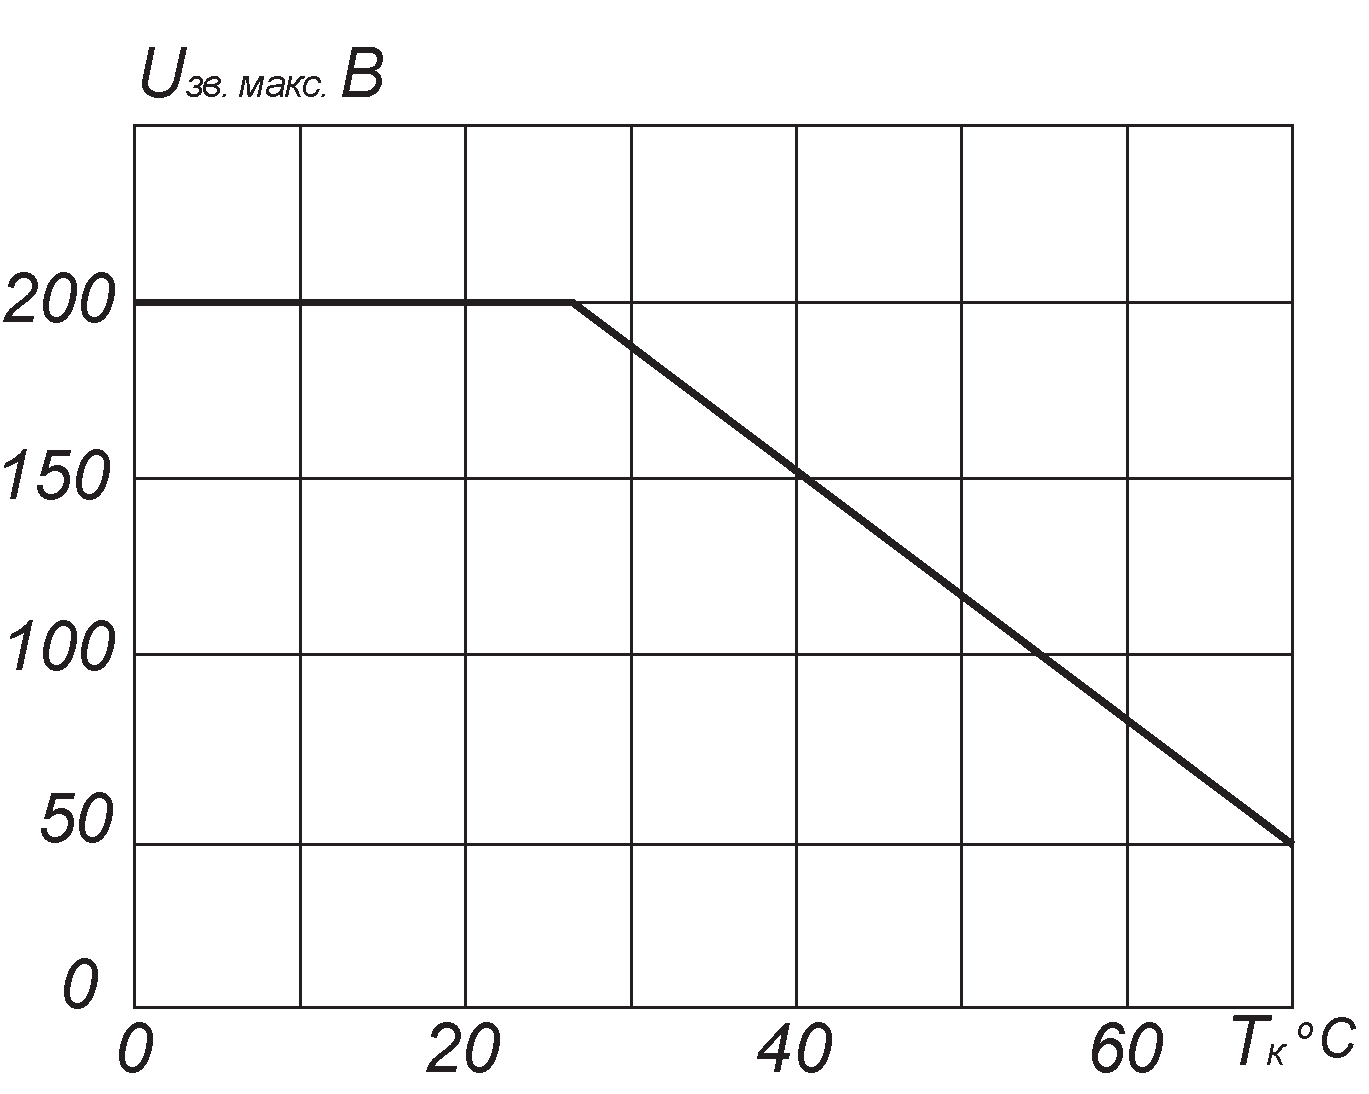
\includegraphics[width=1\linewidth]{1.20.pdf}
    \caption{Залежність допустимої \\зворотної напруги від температури.}
  \end{minipage}
\hfill
  \begin{minipage}[h]{0.5\linewidth}
		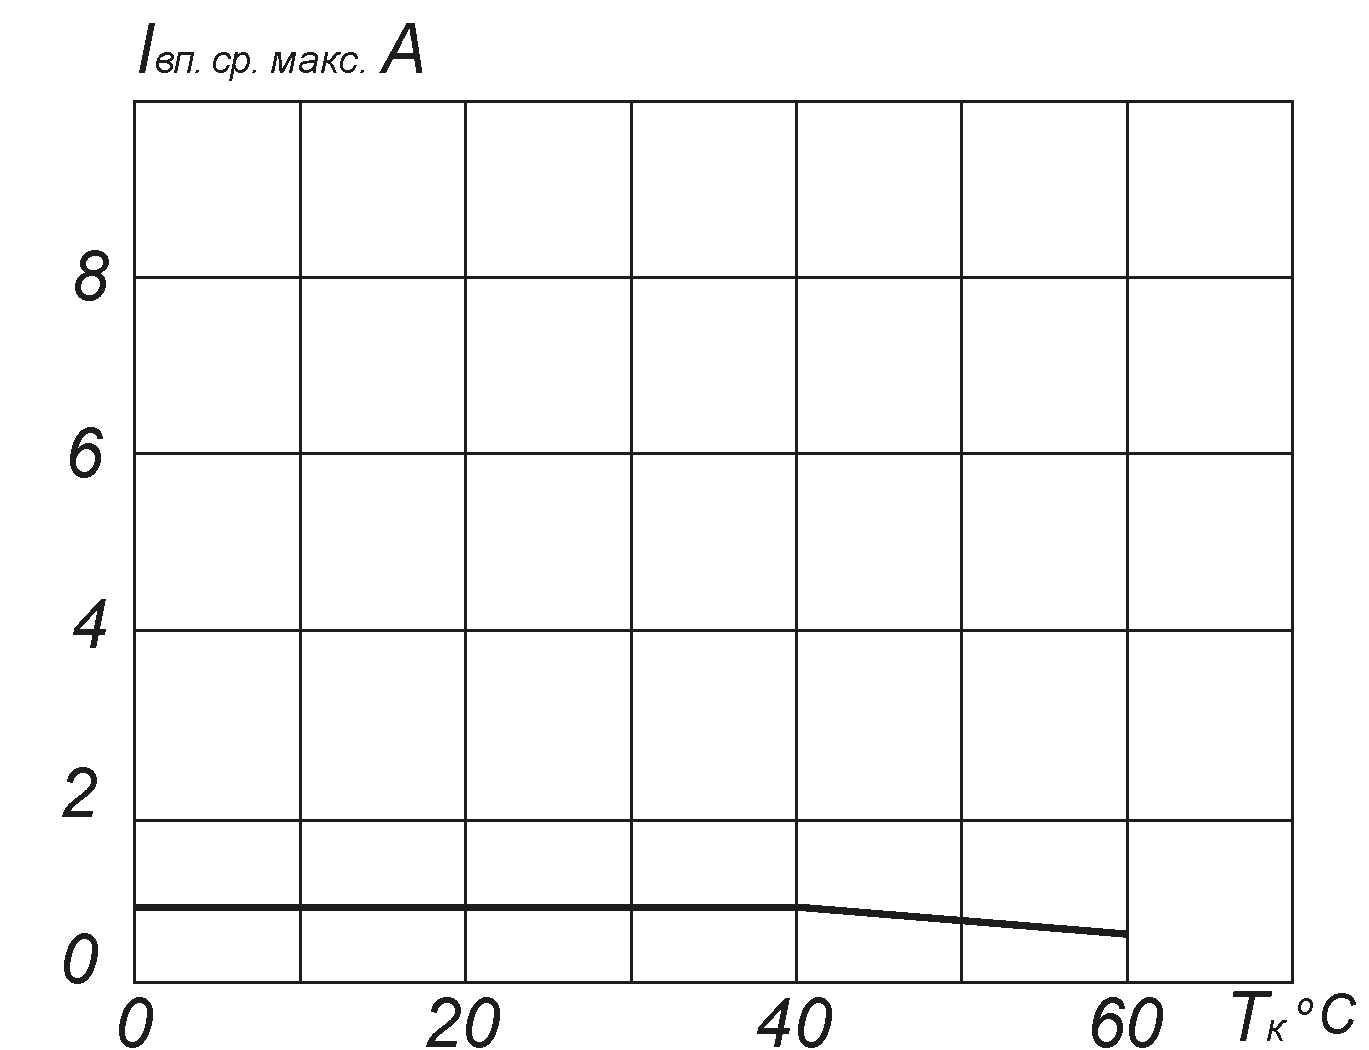
\includegraphics[width=1\linewidth]{1.21.pdf}
    \caption{Залежність допустимого сер-го випрямного струму від температури.}
	\end{minipage}
\end{figure}





%\tcbox[colback=green!5!white, colframe=green!50!black]{asvsdfvsd\\lsidfnb}
  %-----------------------------7---------------------------------
  \newpage
  \section{Імпульсні діоди}
  \begin{tcolorbox}[colback=white!100,colframe=red!75!black,width=19cm,righttitle=0.5cm,subtitle style={boxrule=0.4pt, colback=yellow!50!red!25!white},title= \bf{Графічне позначення}\hfill  \bf{Натуральне зоображення}]
  	\begin{center}\bf{КД513А}\end{center}
  	\tcblower
  	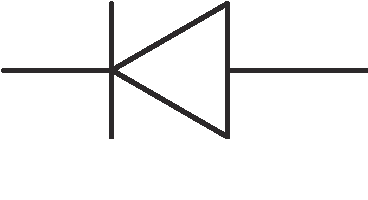
\includegraphics[scale=0.5]{1.1.pdf}\hfill 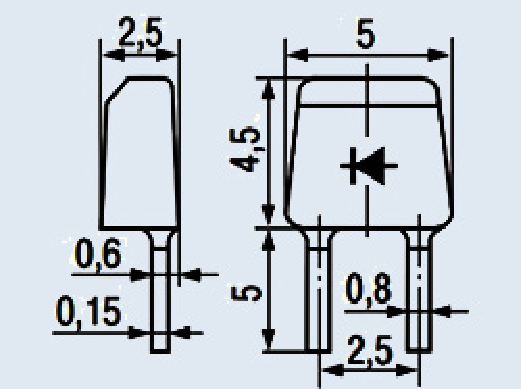
\includegraphics[scale=0.5]{1.2.1.pdf} \hfill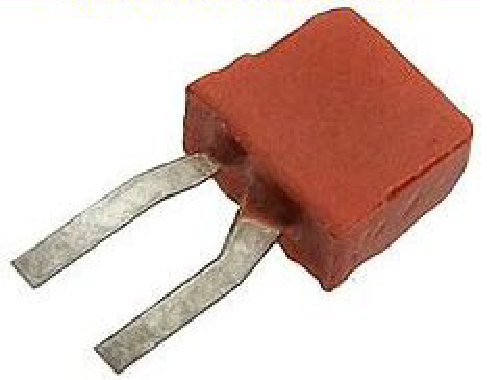
\includegraphics[scale=0.5]{1.2.12.pdf}
  \end{tcolorbox}
  \begin{wrapfigure}[0]{r}{12cm}
  \vspace{-0.7 cm}
  \parbox{12cm}{%
    \begin{tcolorbox}[width=12cm,right=0.5cm]
    Діод КД513А кремнієвий, епітаксіально-планарний, імпульсний.
    Призначений для застосування в імпульсних пристроях наносекундного діапазону. Випускається в пластмасовому корпусі з гнучкими "ніжками". Маса діода не більше 0,11 г. Вигин ніжок допускається не ближче 2 мм.
    \end{tcolorbox}}
  \end{wrapfigure}

  \vspace{0.5 cm}\par
  %\xmybox[green]{$F_{\text{max}}  =    ???????1 \text{ кГц}$}\par
  %\vspace{0.2 cm}\par
  \xmybox[green]{$I_{\text{зв}}   < 5\text{ мкА}$}\par
  \vspace{0.2 cm}\par
  \xmybox[green]{$U_{\text{пр}}       < 1,1\text{ В}$}\par
  \vspace{0.2 cm}\par
  \xmybox[green]{$U_{\text{зв}}  =   50    \text{ В}$}\par
  \vspace{0.2 cm}\par
  \xmybox[green]{$I_{\text{пр}}  =    100 \text{ мА}$}\par
  \vspace{0.2 cm}\par
  \xmybox[green]{$T_{\text{відн. зв.}}  =  0,004 \text{ мкс}$}\par
  \vspace{0.2 cm}\par
  \xmybox[green]{$C_{\text{D}}  =  4 \text{ пФ}$}\par
  \vspace{0.5 cm}\par

  \begin{figure}[h!]\label{im4}
  	\begin{minipage}[h]{0.5\linewidth}
  		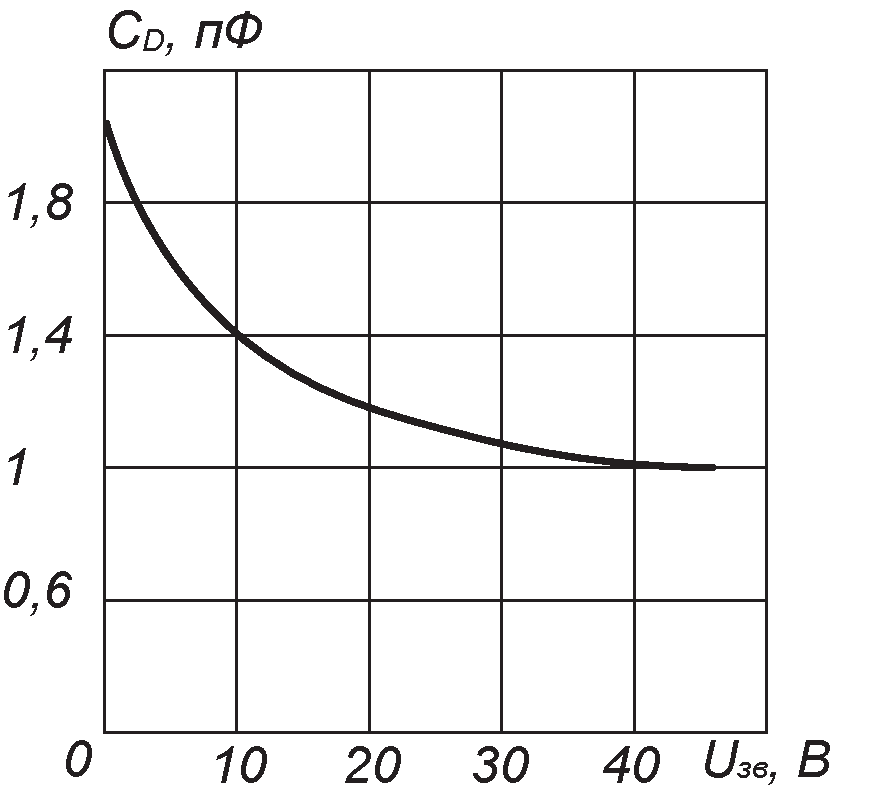
\includegraphics[width=1\linewidth]{1.2.13.pdf}
      \caption{Залежність загальної\\ ємності діода від напруги.}
    \end{minipage}
  \hfill
    \begin{minipage}[h]{0.5\linewidth}
  		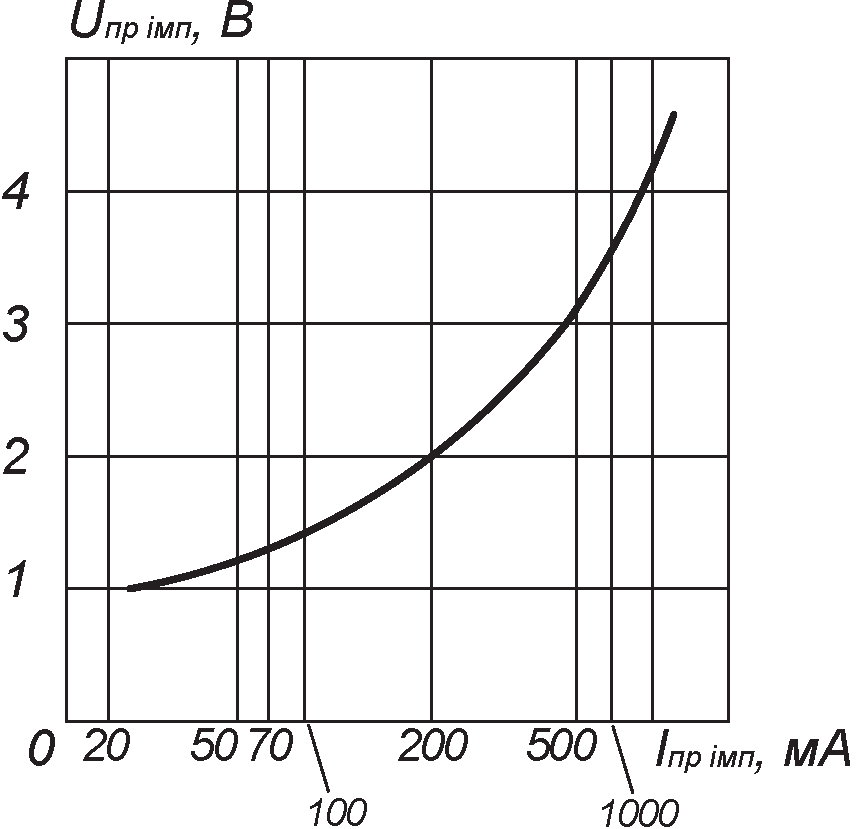
\includegraphics[width=1\linewidth]{1.2.14.pdf}
      \caption{Залежність імпульсної прямої напруги від імпульсного прямого струму.}
  	\end{minipage}
  \end{figure}





  %--------------------------------------------------------------------------------------8-----------------------------------------------------------------------------------------
  \newpage
  \begin{tcolorbox}[colback=white!100,colframe=red!75!black,width=19cm,righttitle=0.5cm,subtitle style={boxrule=0.4pt, colback=yellow!50!red!25!white},title= \bf{Графічне позначення}\hfill  \bf{Натуральне зоображення}]
  	\begin{center}\bf{1N4148}\end{center}
  	\tcblower
  	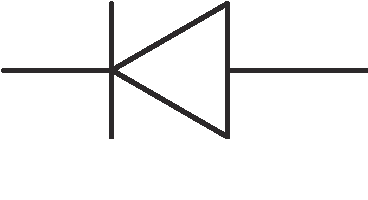
\includegraphics[scale=0.5]{1.1.pdf}\hfill \includegraphics[scale=0.8]{1.2.15.jpg} \hfill\includegraphics[scale=0.2]{1.2.16.jpg}
  \end{tcolorbox}
  \begin{wrapfigure}[0]{r}{12cm}
  \vspace{-0.7 cm}
  \parbox{12cm}{%
    \begin{tcolorbox}[width=12cm,right=0.5cm]
    Діод 1N4148, вагою 0,14г, вельми широко розповсюджений, його аналоги можна виявити практично в будь-якому електронному приладі: від зарядного пристрою телефону до телевізора. Робоча температура складає $-60\ldots+190 \text{ }^{ \circ}C$. Якщо потрібен діод з маленьким зворотним струмом і великою швидкодією, але величина падіння напруги на діоді не принципова, то 1N4148 і його аналоги (КД522Б, LL4148, LS4148) ідеальний вибір.
    \end{tcolorbox}}
  \end{wrapfigure}

  \vspace{0.5 cm}\par
  \xmybox[green]{$I_{\text{зв}}  =  5\text{ мкА}$}\par
  \vspace{0.2 cm}\par
  \xmybox[green]{$U_{\text{пр}}  =    1 \text{ В}$}\par
  \vspace{0.2 cm}\par
  \xmybox[green]{$U_{\text{зв}}  =   75    \text{ В}$}\par
  \vspace{0.2 cm}\par
  \xmybox[green]{$I_{\text{пр}}  =    0,15 \text{ А}$}\par
  \vspace{0.2 cm}\par
  \xmybox[green]{$T_{\text{відн. зв.}}  =  4 \text{ нс}$}\par
  \vspace{0.2 cm}\par
  \xmybox[green]{$C_{\text{D}}  =  4 \text{ пФ}$}\par
  \vspace{0.2 cm}\par
  \xmybox[green]{$I_{\text{пр імп}}  =    0,45 \text{ А}$}\par
  \vspace{0.2 cm}\par
  \xmybox[green]{$P =    500 \text{ мВт}$}\par
  \vspace{0.5 cm}\par

\begin{center}
  \begin{figure}[h!]\label{im5}
  	\center{	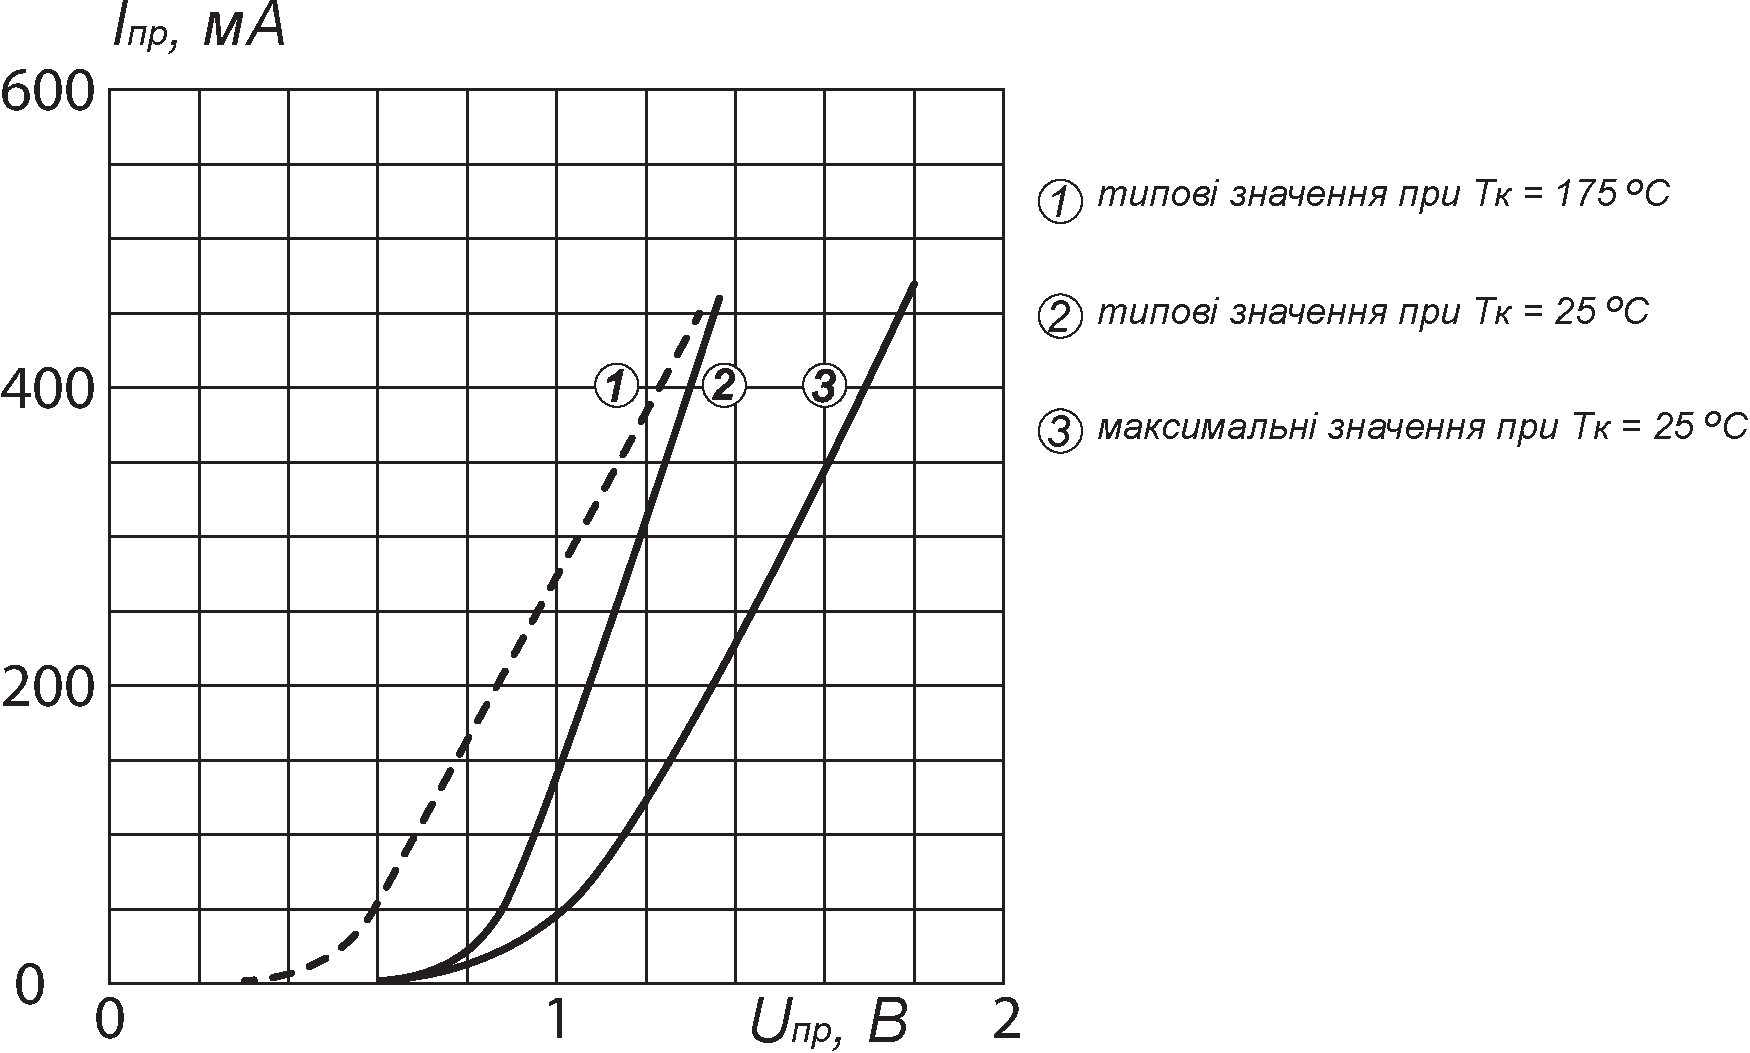
\includegraphics[width=0.85\linewidth]{1.2.18.pdf}}
      \caption{Залежність прямого струму від прямої напруги.}
  \end{figure}
%--------------------------------------------------------------------------------------9----------------------------------------------------------------------------------------
  \begin{figure}[h!]\label{im6}
    \center{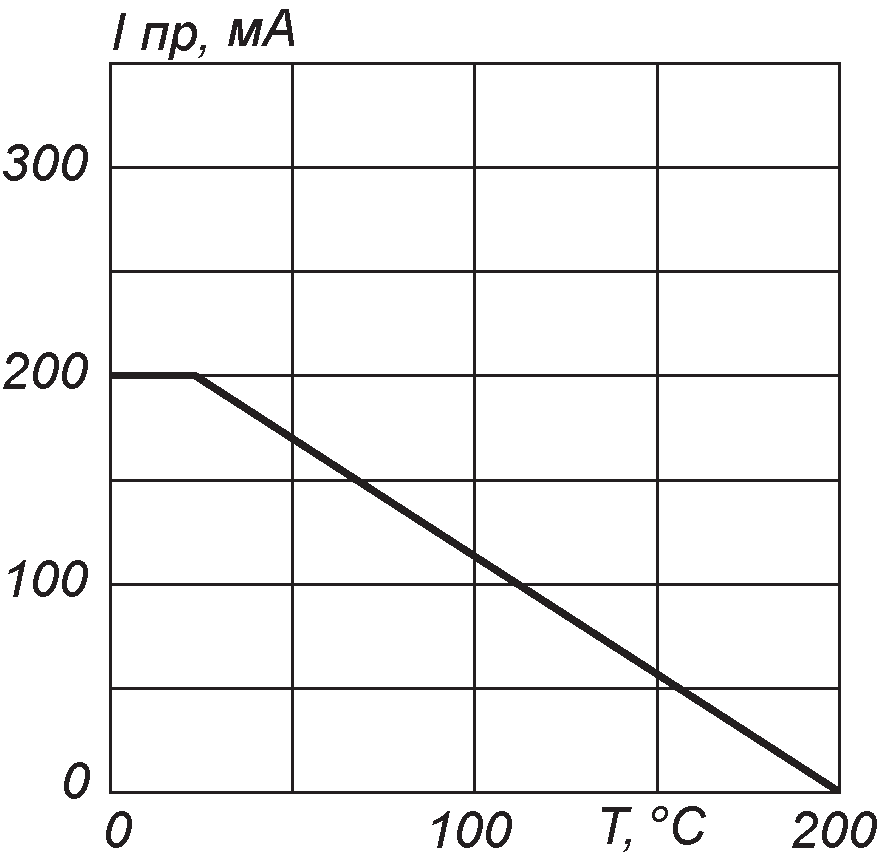
\includegraphics[width=0.5\linewidth]{1.2.17.pdf}}
    \caption{Залежність максимально допустимого неперервного прямого струму від температури навколишнього середовища.}
    \end{figure}
    \begin{figure}[h!]\label{im7}
      \center{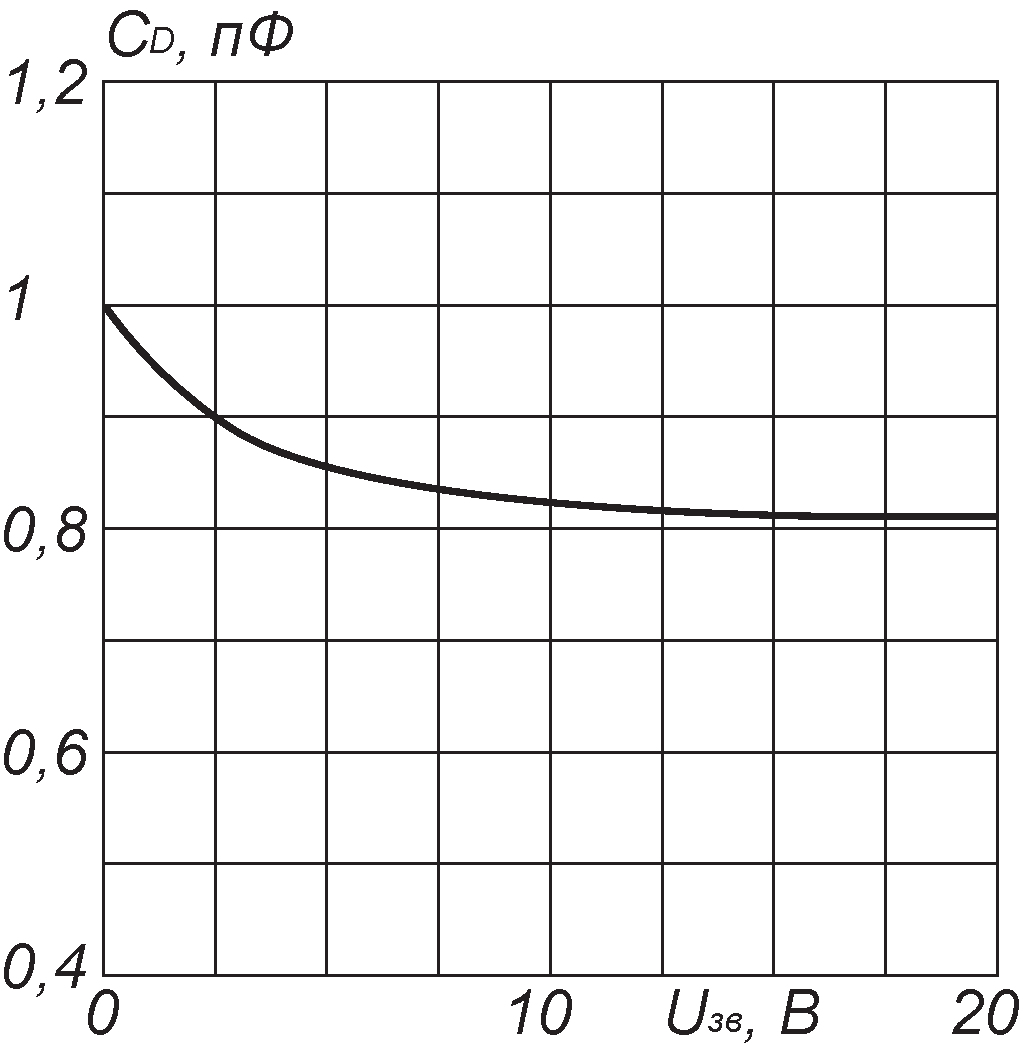
\includegraphics[width=0.5\linewidth]{1.2.19.pdf}}
      \caption{Залежність ємності діода від реверсивної напруги; типові значення при $T=25\text{ }^{\circ}C \text{ та } F_d= \text{ 1МГц}$.}
      \end{figure}
\end{center}
\clearpage
%--------------------------------------------------------------------------------------10-----------------------------------------------------------------------------------------
\section{Стабілітрон і стабістор}
\begin{tcolorbox}[colback=white!100,colframe=red!75!black,width=19cm,righttitle=0.5cm,subtitle style={boxrule=0.4pt, colback=yellow!50!red!25!white},title= \bf{Графічне позначення}\hfill  \bf{Натуральне зоображення}]
  \begin{center}\bf{КС115А}\end{center}
  \tcblower
  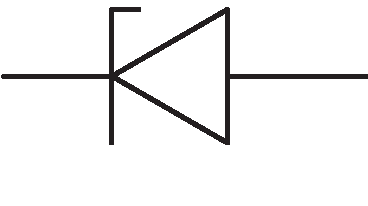
\includegraphics[scale=0.5]{1.3.23.pdf}\hfill \includegraphics[scale=0.7]{1.3.22.pdf} \hfill\includegraphics[scale=0.4]{1.3.24.pdf}
\end{tcolorbox}
\begin{wrapfigure}[0]{r}{12cm}
\vspace{-0.7 cm}
\parbox{12cm}{%
  \begin{tcolorbox}[width=12cm,right=0.5cm]
  Робоча температура складає $-60\ldots+125 \text{ }^{ \circ}C$.
  Стабілітрон КС115А, вагою 0,2г, потрібен для захисту електроапаратури від перенавантаження.
  \end{tcolorbox}}
\end{wrapfigure}

\vspace{0.5 cm}\par
\xmybox[green]{$U_{\text{ст}} =    1,4\ldots 1,6 \text{ В}$}\par
\vspace{0.2 cm}\par
\xmybox[green]{$I_{\text{ст}}  =    1\ldots 100 \text{ мА}$}\par
\vspace{0.2 cm}\par
\xmybox[green]{$P =    	0.26 \text{ Вт}$}\par
\vspace{0.2 cm}\par
\xmybox[green]{$R_{\text{ст}}  =   35    \text{ Ом при } I_{\text{ст}} = 3 \text{ мА}$}\par
\vspace{0.5 cm}\par

\begin{figure}[h!]\label{im7}
  \begin{minipage}[h]{0.5\linewidth}
    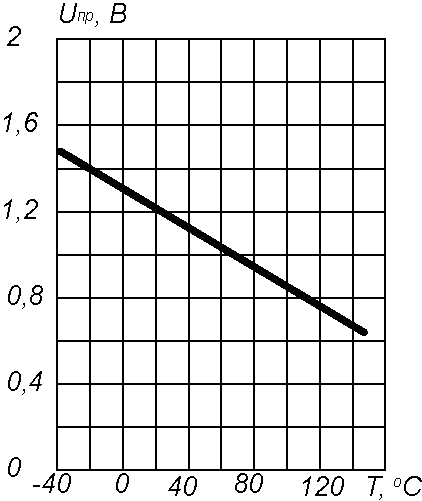
\includegraphics[width=1\linewidth]{1.3.25.pdf}
    \caption{Залежність прямої напруги \\від температури зовнішнього \\середовища.}
  \end{minipage}
\hfill
  \begin{minipage}[h]{0.55\linewidth}
    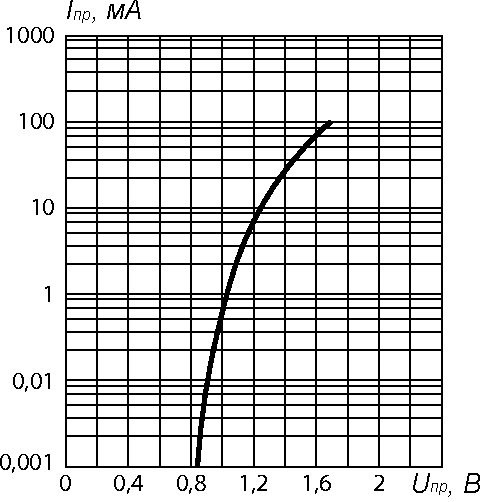
\includegraphics[width=1\linewidth]{1.3.26.pdf}
    \caption{Залежність прямої напруги від прямого струму при температурі $25\text{ }^{\circ}C$.}
  \end{minipage}
\end{figure}

\clearpage
%--------------------------------------------------------------------------------------11-----------------------------------------------------------------------------------------
\begin{tcolorbox}[colback=white!100,colframe=red!75!black,width=19cm,righttitle=0.5cm,subtitle style={boxrule=0.4pt, colback=yellow!50!red!25!white},title= \bf{Графічне позначення}\hfill  \bf{Натуральне зоображення}]
  \begin{center}\bf{Д220С}\end{center}
  \tcblower
  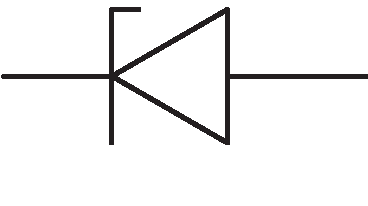
\includegraphics[scale=0.5]{1.3.23.pdf}\hfill \includegraphics[scale=0.4]{1.3.28.png} \hfill\includegraphics[scale=0.35]{1.3.27.pdf}
\end{tcolorbox}
\begin{wrapfigure}[0]{r}{11cm}
\vspace{-0.7 cm}
\parbox{11cm}{%
  \begin{tcolorbox}[width=12cm,right=0.5cm]
  Маса Стабистор не більше 0,5 г. Робоча температура складає $-60\ldots+120 \text{ }^{ \circ}C$.
  Стабістор Д220С кремнієвий, мікросплавний, малої потужності.
Призначений для стабілізації постійної та імпульсної напруги і також обмеження імпульсів напруги. Випускається в скляному корпусі з гнучкими виводами.
  \end{tcolorbox}}
\end{wrapfigure}

\vspace{0.5 cm}\par
\xmybox[green]{$U_{\text{ст}} =    0,59 \text{ В} \text{ при } 1 \text{ мА}$}\par
\vspace{0.2 cm}\par
\xmybox[green]{$U_{\text{ст}} =    1,5 \text{ В} \text{ при } 50 \text{ мА}$}\par
\vspace{0.2 cm}\par
\xmybox[green]{$I_{\text{ст}}  =    1\ldots 50 \text{ мА}$}\par
\vspace{1.5 cm}\par

\begin{figure}[h!]\label{im7}
  \begin{center}
    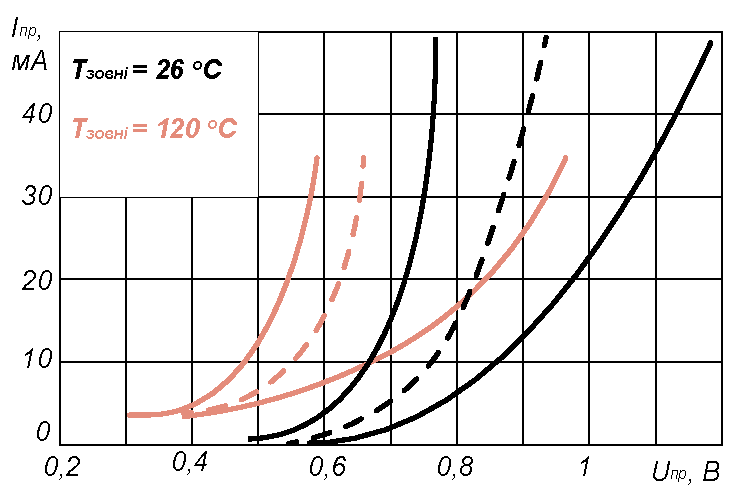
\includegraphics[width=0.9\linewidth]{1.3.29.pdf}
    \caption{Cуцільними лініями показані межі областей, в яких розташовуються вольтамперні характеристики стабістора, а штрихованими лініями їх середнє положення.}
  \end{center}
\end{figure}
\clearpage
%--------------------------------------------------------------------------------------12-----------------------------------------------------------------------------------------
\section{Варикапи}
\begin{tcolorbox}[colback=white!100,colframe=red!75!black,width=19cm,righttitle=0.5cm,subtitle style={boxrule=0.4pt, colback=yellow!50!red!25!white},title= \bf{Графічне позначення}\hfill  \bf{Натуральне зоображення}]
  \begin{center}\bf{КВ109А}\end{center}
  \tcblower
  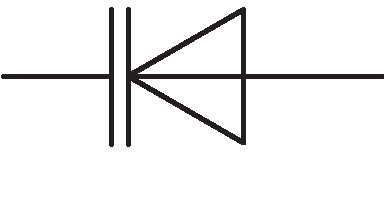
\includegraphics[scale=0.6]{1.4.1.pdf}\hfill \includegraphics[scale=0.7]{1.4.2.pdf} \hfill\includegraphics[scale=0.2]{1.4.3.jpg}
\end{tcolorbox}
\begin{wrapfigure}[0]{r}{12cm}
\vspace{-0.7 cm}
\parbox{12cm}{%
  \begin{tcolorbox}[width=12cm,right=0.5cm]
  Робоча температура складає $-40\ldots+85 \text{ }^{ \circ}C$.
  Маса варикапа не більше 0,06 г. Білою точкою позначають позитивний вивід.


  \end{tcolorbox}}
\end{wrapfigure}

\vspace{0.5 cm}\par
\xmybox[green]{$U_{\text{зв}} =    25 \text{ В}$}\par
\vspace{0.2 cm}\par
\xmybox[green]{$I_{\text{зв}}  =    0,5 \text{ мА}$}\par
\vspace{0.2 cm}\par
\xmybox[green]{$Q_{\text{в}} =    	300 \text{}$}\par
\vspace{0.2 cm}\par
\xmybox[green]{$C_{\text{D}} =    	2,3\ldots 2,8 \text{ пФ}$}\par
\vspace{0.2 cm}\par
\xmybox[green]{$P_{\text{}}  =   5   \text{ мВт}$}\par
\vspace{0.2 cm}\par
\xmybox[green]{$K_{\text{c}}  =   4,0\ldots 5,5  \text{ мВт, при } 3\ldots 25\text{ B}$}\par
\vspace{0.5 cm}\par

\begin{figure}[h!]\label{im7}
  \begin{minipage}[h]{0.5\linewidth}
    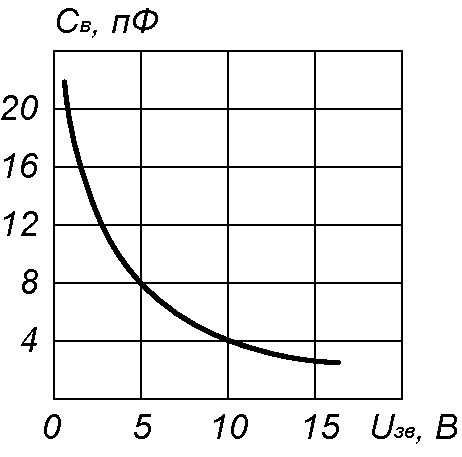
\includegraphics[width=1\linewidth]{1.4.4.pdf}
    \caption{Залежність ємності\\ від напруги.}
  \end{minipage}
\hfill
  \begin{minipage}[h]{0.55\linewidth}
    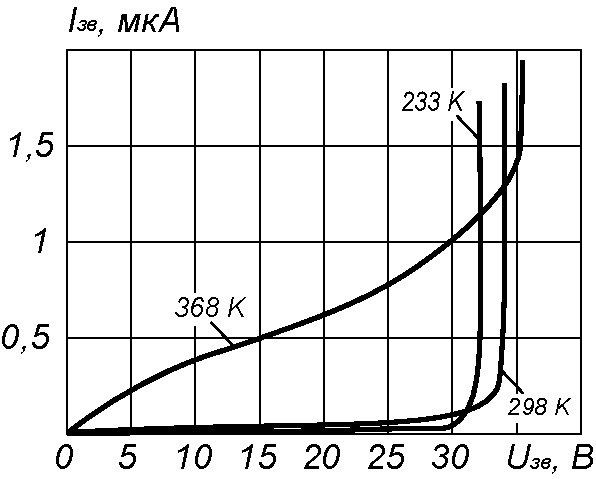
\includegraphics[width=1\linewidth]{1.4.5.pdf}
    \caption{Залежність зворотного струму\\ від напруги.}
  \end{minipage}
\end{figure}

\clearpage
%--------------------------------------------------------------------------------------13-----------------------------------------------------------------------------------------
\begin{tcolorbox}[colback=white!100,colframe=red!75!black,width=19cm,righttitle=0.5cm,subtitle style={boxrule=0.4pt, colback=yellow!50!red!25!white},title= \bf{Графічне позначення}\hfill  \bf{Натуральне зоображення}]
  \begin{center}\bf{Д901Е}\end{center}
  \tcblower
  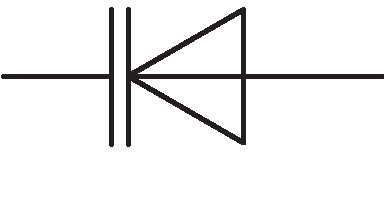
\includegraphics[scale=0.55]{1.4.1.pdf}\hfill \includegraphics[scale=0.17]{1.4.6.png} \hfill\includegraphics[scale=0.3]{1.4.7.pdf}
\end{tcolorbox}
\begin{wrapfigure}[0]{r}{13cm}
\vspace{-0.7 cm}
\parbox{14cm}{%
  \begin{tcolorbox}[width=13.5cm,right=0.5cm]
  Варикап кремнієвий, сплавний, ''подстроечный'', робоча температура $-40\ldots+125 \text{ }^{ \circ}C$.
  Маса не більше 1 г. Добротність на частоті $F = 50$ МГц сягає $Q_{\text{в}}=$ 25.
Призначений для застосування в схемах ''подстраивания'' контурів резонансних підсилювачів.
Випускаються в металлостеклянном корпусі з гнучкими нінжками.

  \end{tcolorbox}}
\end{wrapfigure}

\vspace{0.5 cm}\par
\xmybox[green]{$U_{\text{зв}} =    45 \text{ В}$}\par
\vspace{0.2 cm}\par
\xmybox[green]{$I_{\text{зв}}  =    1 \text{ мА}$}\par
\vspace{0.2 cm}\par
\xmybox[green]{$Q_{\text{в}} =    	30 \text{}$}\par
\vspace{0.2 cm}\par
\xmybox[green]{$C_{\text{D}} =    27 \text{ пФ}$}\par
\vspace{0.2 cm}\par
\xmybox[green]{$P_{\text{}}  =   5   \text{ мВт}$}\par
\vspace{0.2 cm}\par
\xmybox[green]{$K_{\text{c}}  =   3,6\ldots 4,4  \text{ мВт, при } 4\ldots 80\text{ B}$}\par
\vspace{0.5 cm}\par

\begin{figure}[h!]\label{im7}
  \begin{minipage}[h]{0.5\linewidth}
    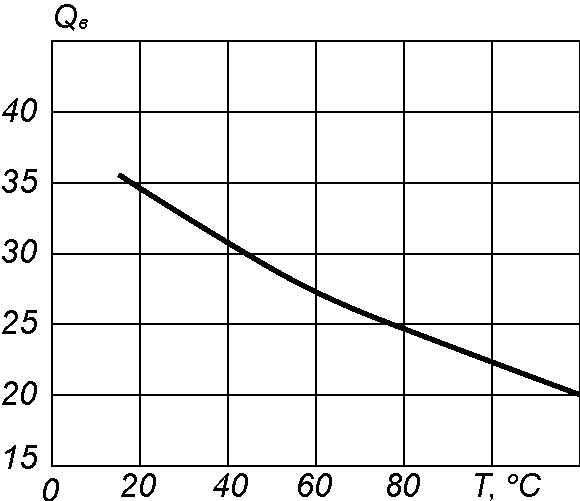
\includegraphics[width=1\linewidth]{1.4.8.pdf}
    \caption{Залежність добротності\\ від температури.}
  \end{minipage}
\hfill
  \begin{minipage}[h]{0.5\linewidth}
    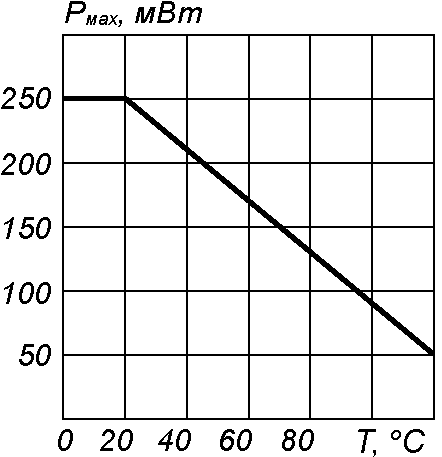
\includegraphics[width=1\linewidth]{1.4.9.pdf}
    \caption{Залежність допустимої розсіювальної потужності, від температури.}
  \end{minipage}
\end{figure}

\clearpage
%--------------------------------------------------------------------------------------14-----------------------------------------------------------------------------------------
\section{Обернений та тунельний  діод}
\begin{tcolorbox}[colback=white!100,colframe=red!75!black,width=19cm,righttitle=0.5cm,subtitle style={boxrule=0.4pt, colback=yellow!50!red!25!white},title= \bf{Графічне позначення}\hfill  \bf{Натуральне зоображення}]
  \begin{center}\bf{3И402А}\end{center}
  \tcblower
  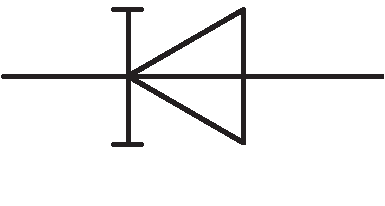
\includegraphics[scale=0.6]{1.5.9.pdf}\hfill \includegraphics[scale=0.7]{1.5.2.pdf} \hfill\includegraphics[scale=0.55]{1.5.3.pdf}
\end{tcolorbox}
\begin{wrapfigure}[0]{r}{12cm}
\vspace{-0.7 cm}
\parbox{12cm}{%
  \begin{tcolorbox}[width=12cm,right=0.5cm]
  Діод арсенідогаліевий, обернений, сплавний, масою не більше 0,15 г. Робоча температура складає $-60\ldots+100 \text{ }^{ \circ}C$.

  Випускається в металлокерамическом корпусі з гнучкими нінжками.


  \end{tcolorbox}}
\end{wrapfigure}

\vspace{0.5 cm}\par
\xmybox[green]{$U_{\text{зв}} =    25 \text{ В}$}\par
\vspace{0.2 cm}\par
\xmybox[green]{$I_{\text{зв}}  =    0,5 \text{ мА}$}\par
\vspace{0.2 cm}\par
\xmybox[green]{$Q_{\text{в}} =    	300 \text{}$}\par
\vspace{0.2 cm}\par
\xmybox[green]{$C_{\text{D}} =    	2,3\ldots 2,8 \text{ пФ}$}\par
\vspace{0.2 cm}\par
\xmybox[green]{$P_{\text{}}  =   5   \text{ мВт}$}\par
\vspace{0.2 cm}\par
\xmybox[green]{$K_{\text{c}}  =   4,0\ldots 5,5  \text{ мВт, при } 3\ldots 25\text{ B}$}\par
\vspace{0.5 cm}\par

\begin{figure}[h!]\label{im8}
  \begin{minipage}[h]{0.5\linewidth}
    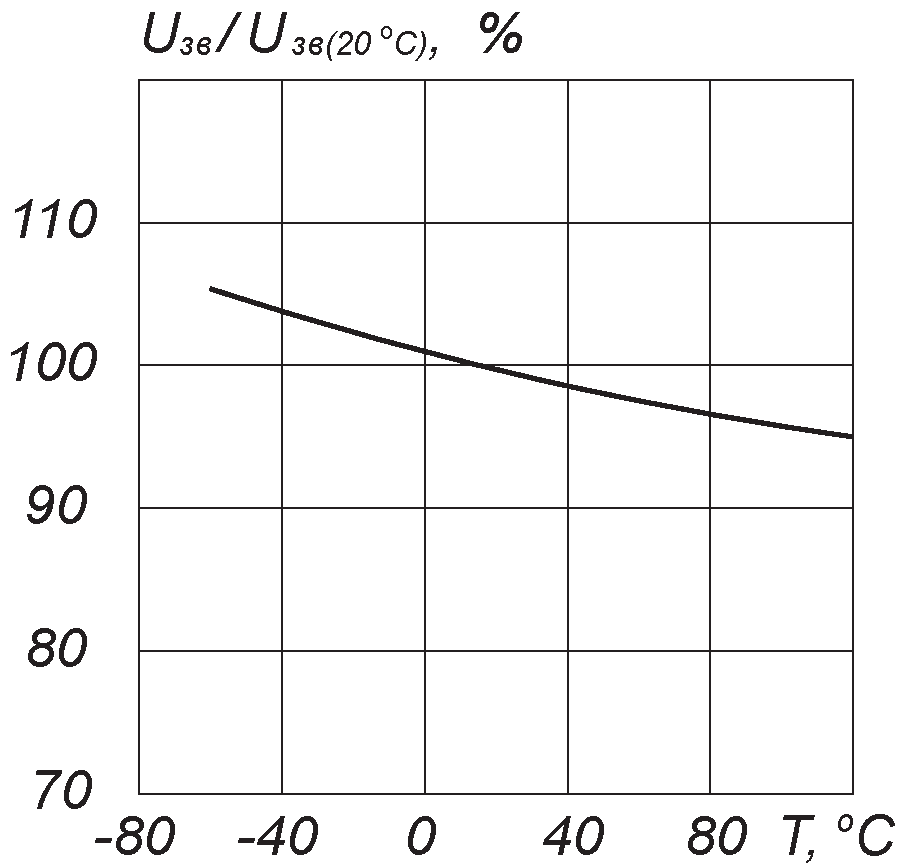
\includegraphics[width=1\linewidth]{1.5.4.pdf}
    \caption{Залежність зворотної\\ напруги від температури.}
  \end{minipage}
\hfill
  \begin{minipage}[h]{0.5\linewidth}
    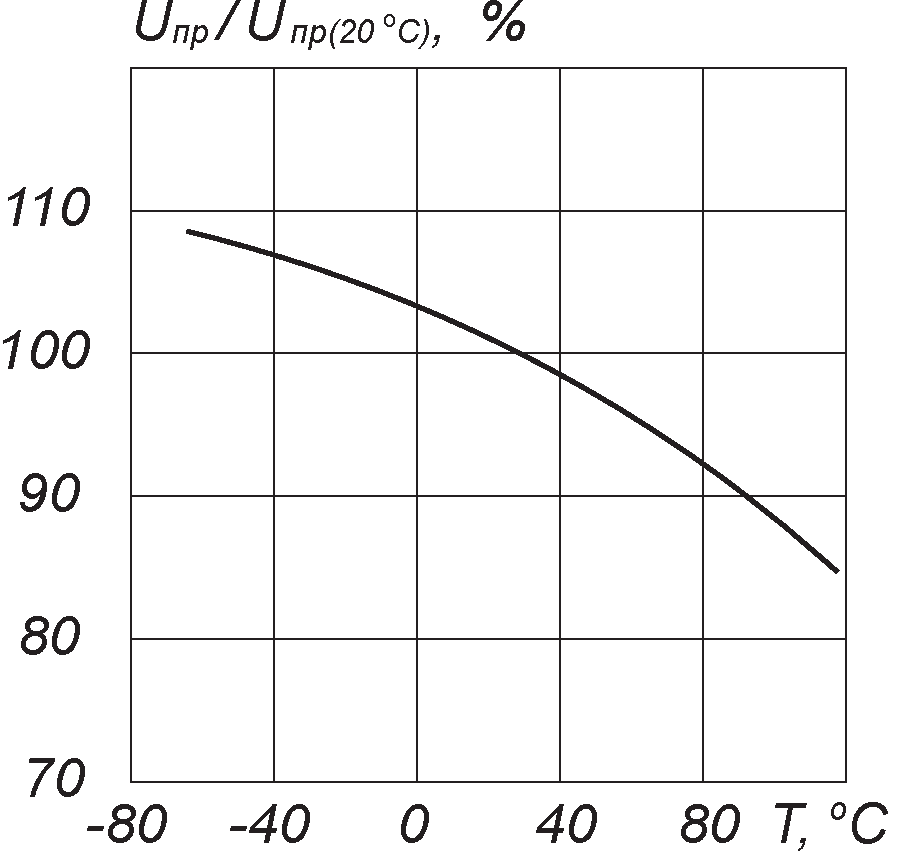
\includegraphics[width=1\linewidth]{1.5.5.pdf}
    \caption{Залежність прямої напруги від температури.}
  \end{minipage}
\end{figure}
%--------------------------------------------------------------------------------------15-----------------------------------------------------------------------------------------

\begin{figure}[h!]\label{im9}
  \begin{minipage}[h]{0.5\linewidth}
    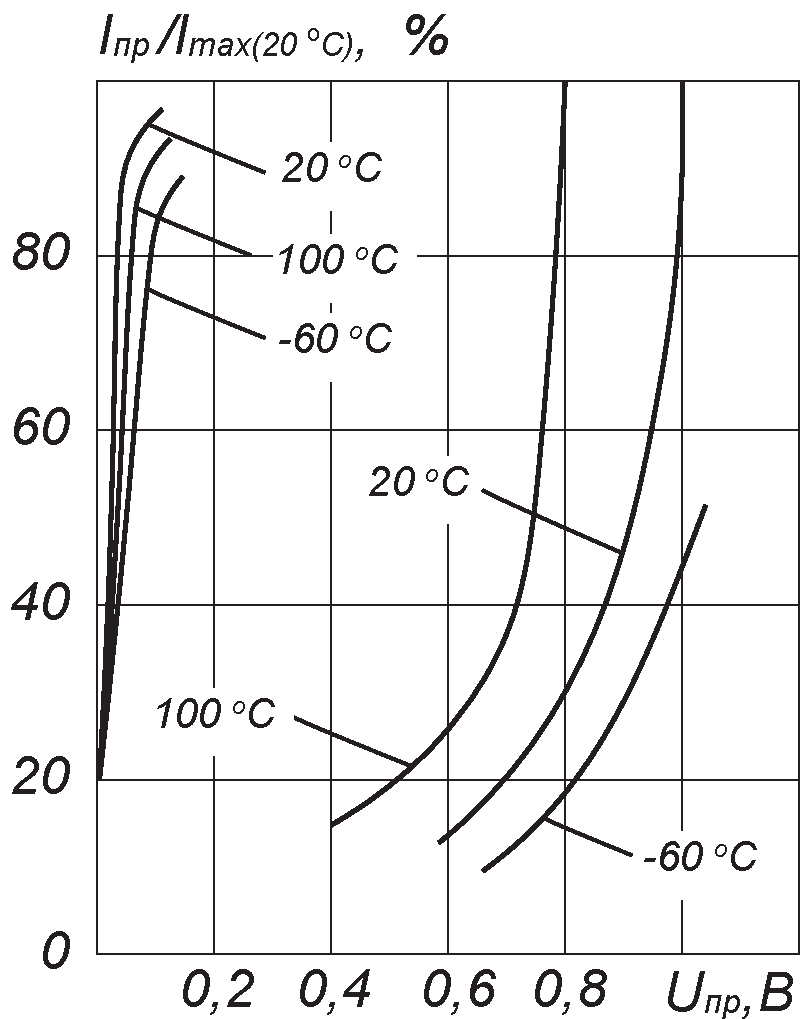
\includegraphics[width=1\linewidth]{1.5.6.pdf}
    \caption{Вольт-амперні характеристики.}
  \end{minipage}
\hfill
  \begin{minipage}[h]{0.43\linewidth}
    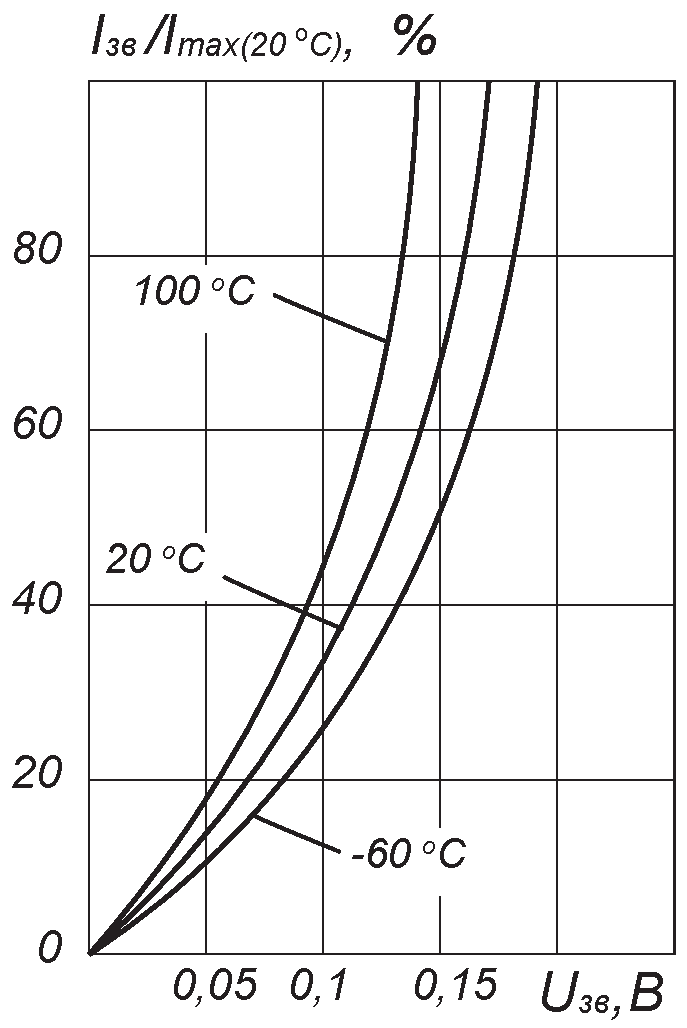
\includegraphics[width=1\linewidth]{1.5.7.pdf}
    \caption{Обернені вольт-амперні характеристики.}
  \end{minipage}
\end{figure}

\begin{figure}[h!]\label{im10}
  \begin{center}
    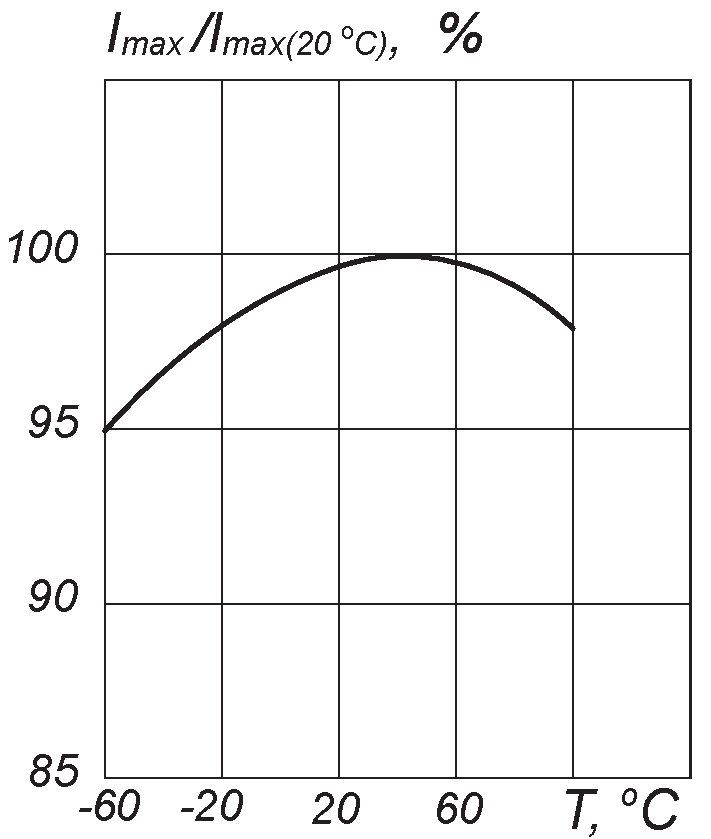
\includegraphics[width=0.44\linewidth]{1.5.8.pdf}
    \caption{Залежність пікового струму від напруги.}
  \end{center}
\end{figure}

\clearpage
%--------------------------------------------------------------------------------------16-----------------------------------------------------------------------------------------
\begin{tcolorbox}[colback=white!100,colframe=red!75!black,width=19cm,righttitle=0.5cm,subtitle style={boxrule=0.4pt, colback=yellow!50!red!25!white},title= \bf{Графічне позначення}\hfill  \bf{Натуральне зоображення}]
  \begin{center}\bf{1N3716}\end{center}
  \tcblower
  \includegraphics[scale=0.6]{1.5.1.pdf}\hfill \includegraphics[scale=0.3]{1.5.10.pdf} \hfill\includegraphics[scale=1.5]{1.5.11.pdf}
\end{tcolorbox}
\begin{wrapfigure}[0]{r}{12cm}
\vspace{-0.7 cm}
\parbox{12cm}{%
  \begin{tcolorbox}[width=12cm,right=0.5cm]
  Діод арсенідогаліевий, обернений, сплавний, масою не більше 0,15 г. Робоча температура складає $-60\ldots+100 \text{ }^{ \circ}C$./?????????????????????????????????????
  Призначений для застосування в детекторах та змішувачах.
  Випускається в металлокерамическом корпусі з гнучкими нінжками.


  \end{tcolorbox}}
\end{wrapfigure}

\vspace{0.5 cm}\par
\xmybox[green]{$U_{\text{зв}}   \leqslant 500 \text{ мВ}$}\par
\vspace{0.2 cm}\par
\xmybox[green]{$I_{\text{}}  = 1\ldots 4,7\text{ мА}$}\par
\vspace{0.2 cm}\par
\xmybox[green]{$R_{\text{}} =    	2 \text{ Ом}$}\par
\vspace{0.2 cm}\par
\xmybox[green]{$C_{\text{D}} =    	50 \text{ пФ}$}\par
\vspace{0.2 cm}\par
\xmybox[green]{$U_{\text{ном}} =    65 \text{ мВ}$}\par
\vspace{0.2 cm}\par
\xmybox[green]{$F_{\text{max}} =    1,8 \text{ ГГц}$}\par
\vspace{0.5 cm}\par

\begin{figure}[h!]\label{im8}
  \begin{minipage}[h]{0.5\linewidth}
    \includegraphics[width=1\linewidth]{1.5.4.pdf}
    \caption{Залежність зворотної\\ напруги від температури.}
  \end{minipage}
\hfill
  \begin{minipage}[h]{0.5\linewidth}
    \includegraphics[width=1\linewidth]{1.5.4.pdf}
    \caption{Залежність прямої напруги від температури.}
  \end{minipage}
\end{figure}

\clearpage
%--------------------------------------------------------------------------------------17-----------------------------------------------------------------------------------------











\newpage
The \xmybox[green]{quick} brown \xmybox{fox} \xmybox[blue]{jumps} over the \xmybox[green]{lazy} \xmybox{dog}.




  %---------------------------------------------------------------------Список використаної літератури------------------------------------------------------------------------------------
\newpage
\begin{thebibliography}{9}
	\bibitem{lit1} wefvnfjnvdlrfbvndfg2009.
\end{thebibliography}

\end{document}
